% Provenance (never printed): see sources/outline_sources.md (Year 3:
% spectral signatures; optical, thermal and radar sensors; radar
% interferometry; digital elevation models; GIS operations).
% Brief: sources/book5/BRIEFS.md, ch. 25. Curves from figdata/bachelor-3/
% spectral_signatures.py (ECOSTRESS spectra and the Landsat 8 OLI bands),
% thermal_ir.py (Planck's law, brightness temperatures, a mixed pixel),
% insar_mogi.py (the wrapped interferogram of a Mogi source) and
% varden_gis.py (slope, aspect and an overlay on the Varden Hills, from
% figdata/shared/region.py, read only). Exercise and problem values in the
% Book 5 scratch calculator calc/ch25.py. Mount Halvren, its lava flows and
% its fumaroles are invented. The brief's overlay (slope > 15 degrees on
% limestone within 200 m of the river) is empty on the Varden model: the
% valley floor is flat; the printed overlay uses the shale within 1 km.
\chapter{Penginderaan Jauh dan SIG}\label{ch:b3:remote-sensing-gis}

Pada 1997 tanah di sebuah kawasan alam liar di Pegunungan Cascade, dekat gugus
gunung api yang disebut Three Sisters, mulai naik. Pada 2001 bagian tengahnya berada
\qty{15}{cm} lebih tinggi. Tidak ada gunung api yang berdiri tepat di atas penggelembungan itu, dan
letusan terakhir di kawasan itu terjadi 1500 tahun lalu. Pengangkatan itu tidak
ditemukan oleh siapa pun yang berjalan di atasnya: ia tampak sebagai sasaran cincin berwarna ketika
citra radar kawasan itu, diambil dari orbit selang beberapa tahun, digabungkan.
Cincin-cincin itu menempatkan magma yang menyusup pada kedalaman 6 sampai \qty{7}{km}; pada Maret 2004
rentetan lebih dari 300 gempa bumi kecil melanda tepat di dekat pusatnya.
Bab ini menjelaskan bagaimana satelit mengukur perubahan beberapa sentimeter dari
ketinggian ratusan kilometer, apa yang dilihat sensor lain di orbit tentang permukaan
tanah, dan bagaimana peta yang dihasilkan sensor-sensor itu digabungkan
dalam sistem informasi geografis.
% ledger: usgs:insar-fs

\begin{recall}
Spektrum elektromagnetik, hukum Planck tentang benda hitam, emisivitas
dan hukum Kirchhoff, reflektansi, dan interferensi gelombang dibahas dalam
buku fisika. Penginderaan jauh, citra satelit, proyeksi peta, dan
penentuan posisi dengan satelit dibahas dalam volume-volume sekolah. Jendela atmosfer dan
pita fotometrik dibahas dalam volume Tahun 1, pada bab tentang teleskop;
model elevasi digital dan sistem informasi geografis yang menyimpannya, pada
bab tentang peta geologi; peta radar pertama tentang pergeseran akibat
gempa bumi, pada bab tentang sumber gempa. Sumber Mogi dari reservoir magma
yang menggelembung dibahas dalam volume Tahun 2, pada
bab tentang letusan gunung api.
\end{recall}

\section{Tanda spektral dan sensor optik}\label{sec:b3:remote-sensing-gis:optical}

Sinar Matahari yang mencapai permukaan tanah sebagian diserap dan sebagian
dipantulkan, dengan proporsi yang bergantung pada panjang gelombang dan pada
bahan penyusun tanah. Sensor di orbit mengukur cahaya pantulan dalam beberapa
rentang panjang gelombang, yaitu pitanya, dan rasio antarpita itu mengidentifikasi
permukaan.

\begin{definition}[Tanda spektral]\label{def:b3:remote-sensing-gis:signature}
Yang disebut \emph{tanda spektral}\index{tanda spektral} suatu bahan adalah
reflektansinya sebagai fungsi panjang gelombang, $R(\lambda)$, yaitu pecahan
radiasi datang yang dipantulkannya. Pada inframerah termal, tempat permukaan
memancarkan alih-alih memantulkan, tanda spektralnya adalah emisivitas
$\varepsilon(\lambda)$; untuk sampel buram $\varepsilon = 1 - R$.
\end{definition}

\begin{omfigure}
\centering
\begin{tikzpicture}
\begin{axis}[width=0.9\linewidth, height=6.4cm, xmin=0.4, xmax=2.5, ymin=0, ymax=1,
  xlabel={panjang gelombang (\unit{\micro\metre})}, ylabel={reflektansi},
  tick label style={font=\scriptsize}, label style={font=\small},
  legend style={font=\scriptsize, at={(0.5,-0.24)}, anchor=north, /tikz/every even column/.append style={column sep=4pt}},
  legend columns=5, clip=false]
\fill[black!8] (axis cs:0.45,0) rectangle (axis cs:0.51,1);
\fill[black!8] (axis cs:0.53,0) rectangle (axis cs:0.59,1);
\fill[black!8] (axis cs:0.64,0) rectangle (axis cs:0.67,1);
\fill[black!8] (axis cs:0.85,0) rectangle (axis cs:0.88,1);
\fill[black!8] (axis cs:1.57,0) rectangle (axis cs:1.65,1);
\fill[black!8] (axis cs:2.11,0) rectangle (axis cs:2.29,1);
\addplot[very thick, green!50!black] table[x=um, y=grass] {figdata/out/bachelor-3-spectral_signatures-spectra.dat};
\addlegendentry{rumput hijau}
\addplot[thick, brown!70!black, dashed] table[x=um, y=soil] {figdata/out/bachelor-3-spectral_signatures-spectra.dat};
\addlegendentry{tanah pasir cokelat}
\addplot[thick, black!55] table[x=um, y=kaol] {figdata/out/bachelor-3-spectral_signatures-spectra.dat};
\addlegendentry{kaolinit}
\addplot[thick, red!70!black, dash dot] table[x=um, y=hem] {figdata/out/bachelor-3-spectral_signatures-spectra.dat};
\addlegendentry{hematit}
\addplot[thick, omDef] table[x=um, y=water] {figdata/out/bachelor-3-spectral_signatures-spectra.dat};
\addlegendentry{air}
\node[font=\tiny, anchor=south] at (axis cs:0.48,1) {2};
\node[font=\tiny, anchor=south] at (axis cs:0.56,1) {3};
\node[font=\tiny, anchor=south] at (axis cs:0.655,1) {4};
\node[font=\tiny, anchor=south] at (axis cs:0.865,1) {5};
\node[font=\tiny, anchor=south] at (axis cs:1.61,1) {6};
\node[font=\tiny, anchor=south] at (axis cs:2.2,1) {7};
\end{axis}
\end{tikzpicture}
\par\smallskip{\small Spektrum reflektansi laboratorium lima permukaan (ECOSTRESS
Spectral Library, direproduksi atas izin dari Jet Propulsion
Laboratory, California Institute of Technology), dengan enam pita pantul
pita 2 sampai 7 pencitra Landsat~8 dan 9 diarsir. Rumput hijau gelap di
cahaya tampak, dan paling terang di inframerah dekat; kaolinit terang di seluruh rentang
kecuali serapan sempit pada \qty{2.2}{\micro\metre}; hematit menyerap
biru dan hijau serta memantulkan merah; air memantulkan beberapa persen pada
setiap panjang gelombang.}\label{fig:b3:remote-sensing-gis:spectra}
\end{omfigure}
% ledger: data:b5-ecostress, usgs:landsat8-bands, nasa:ndvi

\omterm{def:b3:remote-sensing-gis:signature}{Tanda spektral} pada gambar di atas adalah kosakata penginderaan jauh
optik. Klorofil daun menyerap kuat antara 0.4 dan
\qty{0.7}{\micro\metre}, untuk fotosintesis, sementara sel-sel daun
memantulkan kuat antara 0.7 dan \qty{1.1}{\micro\metre}: rumput hijau
memantulkan \qty{5}{\percent} cahaya merah pita~4 dan \qty{50}{\percent}
inframerah dekat pita~5, lonjakan yang tak pernah dihasilkan batuan atau tanah. Di luar itu, dua
cekungan dalam di dekat 1.4 dan \qty{1.9}{\micro\metre} adalah tempat air cair
menyerap. Pasir cokelat makin terang secara bertahap ke arah inframerah. Kaolinit,
mineral lempung, putih di cahaya tampak dan memiliki serapan sempit pada
\qty{2.20}{\micro\metre}, di dalam pita~7, yang membuatnya lebih gelap di sana daripada
di pita~6; \omterm{def:b3:remote-sensing-gis:sensors}{sensor hiperspektral} merinci bentuk serapannya dan membedakan satu
lempung dari yang lain. Hematit menyerap biru dan hijau: maka ia tampak merah.
% ledger: nasa:ndvi, data:b5-ecostress

\begin{definition}[Resolusi spasial, spektral dan radiometrik; waktu kunjungan ulang]\label{def:b3:remote-sensing-gis:resolutions}
Yang disebut \emph{resolusi spasial}\index{resolusi spasial} suatu citra ialah
ukuran di permukaan tanah dari satu pikselnya. Adapun \emph{resolusi
spektral}\index{resolusi spektral} ialah jumlah dan lebar pitanya,
sedangkan \emph{resolusi radiometrik}\index{resolusi radiometrik} ialah
jumlah tingkat tempat setiap pengukuran dicatat, yakni $2^b$ untuk $b$ bit.
Sementara itu, \emph{waktu kunjungan ulang}\index{waktu kunjungan ulang} satelit ialah
selang waktu antara dua pengamatannya atas tempat yang sama.
\end{definition}

Keempatnya tidak dapat semuanya tajam sekaligus: piksel yang lebih kecil dan pita yang lebih sempit
masing-masing menangkap lebih sedikit cahaya, dan jalur pindai sempit butuh waktu lebih lama untuk
meliput seluruh Bumi. Pencitra Landsat~8, yang diluncurkan pada 2013, memiliki sembilan pita, sebagian besar
dengan piksel \qty{30}{m} dan satu pita pankromatik pada \qty{15}{m}; ia
merekam 4096 tingkat (12 bit), sedangkan instrumen Landsat 1 sampai 7
merekam 256 tingkat. Dari orbit sinkron-Matahari setinggi \qty{705}{km}, ia mencitrakan
sebuah jalur selebar \qty{185}{km} dan kembali ke tempat yang sama setiap 16 hari;
Landsat~9, di orbit yang sama dengan selisih 8 hari, memangkas separuh waktu tunggu. Pencitra
multispektral tiap satelit Sentinel-2 memiliki 13 pita, pada 10, 20
atau \qty{60}{m}, dengan jalur selebar \qty{290}{km}; dengan dua satelit di
orbit yang sama, kunjungan ulang di khatulistiwa ialah 5 hari.
% ledger: usgs:landsat8-bands, usgs:landsat8-orbit, esa:s2-msi, esa:s2-orbit

\begin{definition}[Sensor multispektral dan hiperspektral]\label{def:b3:remote-sensing-gis:sensors}
Yang disebut \emph{sensor multispektral}\index{sensor multispektral} merekam beberapa
hingga beberapa puluh pita, dipisahkan oleh jeda. Adapun \emph{sensor
hiperspektral}\index{sensor hiperspektral} merekam banyak pita sempit yang berdampingan,
sehingga setiap piksel membawa spektrum yang hampir kontinu, yang dapat
dibandingkan dengan pustaka seperti yang ditampilkan pada gambar di atas.
\end{definition}

Di antara permukaan tanah dan sensor terdapat atmosfer. Atmosfer menghamburkan cahaya
Matahari ke sensor yang tidak pernah menyentuh permukaan tanah, terutama pada
panjang gelombang pendek, yaitu radiansi lintasan, dan ia menyerap sebagian dari apa yang
dipantulkan permukaan di luar jendela atmosfer.

\begin{definition}[Koreksi atmosfer]\label{def:b3:remote-sensing-gis:atm-correction}
Yang disebut \emph{koreksi atmosfer}\index{koreksi atmosfer} ialah
konversi radiansi yang diukur di puncak atmosfer menjadi
reflektansi permukaan, dengan menghilangkan radiansi lintasan dan mengompensasi
serapan sepanjang dua lintasan cahaya, turun dan naik.
\end{definition}

Koreksi paling sederhana mengurangi di tiap pita nilai piksel yang paling
gelap dalam adegan, yakni air jernih yang dalam atau bayangan, yang seharusnya memantulkan
hampir nol: yang mereka tampilkan ialah radiansi lintasan. Koreksi yang cermat
memodelkan molekul, aerosol, dan uap air atmosfer.

\begin{definition}[Indeks vegetasi perbedaan ternormalisasi]\label{def:b3:remote-sensing-gis:ndvi}
Yang disebut \emph{indeks vegetasi perbedaan
ternormalisasi}\index{indeks vegetasi perbedaan ternormalisasi} (NDVI) dari suatu piksel ialah
\[
\mathrm{NDVI} = \frac{R_\mathrm{NIR} - R_\mathrm{red}}{R_\mathrm{NIR} + R_\mathrm{red}} ,
\]
dihitung dari reflektansinya pada pita inframerah dekat dan pita merah.
\end{definition}

Indeks ini berada di antara $-1$ dan $+1$. Tanah tanpa daun hijau memberi nilai
mendekati nol: batuan gundul, pasir, atau salju \num{0.1} ke bawah,
semak dan padang rumput 0.2 sampai 0.3, hutan hujan beriklim sedang dan tropis 0.6 sampai
0.8; daun hijau yang paling rapat mendekati 0.8 sampai 0.9. Dari spektrum pada
gambar di atas, melalui pita 4 dan 5, rumput memberi 0.82, pasir cokelat
0.15 dan air $-0.01$. Sebagai rasio, indeks ini tidak berubah jika
kedua pita diredupkan dalam proporsi yang sama, misalnya oleh lereng yang membelakangi
cahaya atau kabut tipis yang merata: indeks ini mengukur vegetasi, bukan
pencahayaan. Radiansi lintasan aditif, yang lebih besar di pita merah, memang mengubahnya,
itulah sebabnya indeks dihitung dari reflektansi yang sudah terkoreksi
(\cref{exo:b3:remote-sensing-gis:12}).
% ledger: nasa:ndvi, data:b5-ecostress

\section{Inframerah termal}\label{sec:b3:remote-sensing-gis:thermal}

Pada suhu permukaan tanah, sekitar \qty{300}{K}, hukum Planck menempatkan
puncak emisi benda hitam di dekat \qty{9.7}{\micro\metre}, di dalam
jendela atmosfer inframerah termal. Di sana sensor mengukur apa yang
dipancarkan permukaan, bukan yang dipantulkannya. Sensor termal Landsat~8
memiliki dua pita, 10.6 sampai 11.19 dan 11.5 sampai \qty{12.51}{\micro\metre}, dengan
piksel \qty{100}{m}.
% ledger: const:h, const:c, const:kB, usgs:landsat8-bands

\begin{definition}[Suhu kecerahan]\label{def:b3:remote-sensing-gis:brightness}
Yang disebut \emph{suhu kecerahan}\index{suhu kecerahan} $T_b$ suatu
permukaan pada panjang gelombang $\lambda$ ialah suhu benda hitam
yang akan memancarkan radiansi spektral $L$ yang diukur darinya pada
panjang gelombang itu. Yang disebut \emph{suhu kinetik} ialah suhu termodinamika permukaan,
yakni suhu yang akan dibaca termometer.
\end{definition}

\begin{proposition}[Suhu kecerahan dari radiansi]\label{prop:b3:remote-sensing-gis:planck-inversion}
Dengan $c_1 = 2hc^2$ dan $c_2 = hc/k$, radiansi spektral $L$ pada
panjang gelombang $\lambda$ memiliki \omterm{def:b3:remote-sensing-gis:brightness}{suhu kecerahan}
\[
T_b = \frac{c_2}{\lambda \ln\!\left(1 + \dfrac{c_1}{\lambda^5 L}\right)} .
\]
Permukaan dengan emisivitas $\varepsilon < 1$ pada suhu kinetik $T$
memancarkan $L = \varepsilon B_\lambda(T)$ dan memiliki $T_b < T$.
\end{proposition}

\begin{proof}
Hukum Planck memberikan $B_\lambda(T) = c_1\lambda^{-5}/(e^{c_2/\lambda T} -
1)$. Dengan menetapkan $B_\lambda(T_b) = L$ dan menyelesaikannya, $e^{c_2/\lambda T_b} = 1 +
c_1/(\lambda^5L)$, yakni rumus tersebut. $B_\lambda$ bertambah seiring dengan
suhu, sehingga $\varepsilon B_\lambda(T) < B_\lambda(T)$ berakibat $T_b < T$.
\end{proof}
% ledger: const:h, const:c, const:kB

Selisih ini penting. Di pusat pita~10, \qty{10.9}{\micro\metre},
permukaan pada \qty{300}{K} dengan emisivitas 0.95 memiliki \omterm{def:b3:remote-sensing-gis:brightness}{suhu
kecerahan} \qty{296.6}{K}, dan untuk 0.99 \qty{299.3}{K}: satu persen
emisivitas bernilai lebih dari setengah kelvin. Spektrum laboratorium memberikan,
di pita~10, emisivitas 0.98 untuk rumput, 0.99 untuk air, dan
0.97 untuk pasir cokelat. Pemetaan suhu dari orbit karena itu memerlukan
emisivitas setiap piksel, serta koreksi untuk emisi dan
serapan udara di antaranya.
% ledger: data:b5-ecostress

\begin{omfigure}
\centering
\begin{tikzpicture}
\begin{groupplot}[group style={group size=2 by 1, horizontal sep=1.5cm},
  width=0.48\linewidth, height=0.42\linewidth,
  tick label style={font=\scriptsize}, label style={font=\small}, title style={font=\small}]
\nextgroupplot[title={radiansi benda hitam}, xmode=log, ymode=log, xmin=1, xmax=25,
  ymin=0.01, ymax=1e5, xlabel={panjang gelombang (\unit{\micro\metre})},
  ylabel={$B_\lambda$ (\unit{W.m^{-2}.sr^{-1}.\micro\metre^{-1}})},
  xtick={1,2,5,10,20}, xticklabels={1,2,5,10,20}]
\fill[black!10] (axis cs:10.6,0.01) rectangle (axis cs:11.19,1e5);
\fill[black!10] (axis cs:2.11,0.01) rectangle (axis cs:2.29,1e5);
\addplot[thick, omDef] table[x=um, y=b300] {figdata/out/bachelor-3-thermal_ir-planck.dat};
\addplot[thick, omDef, dashed] table[x=um, y=b400] {figdata/out/bachelor-3-thermal_ir-planck.dat};
\addplot[thick, red!70!black] table[x=um, y=b1443] {figdata/out/bachelor-3-thermal_ir-planck.dat};
\node[font=\scriptsize, omDef, anchor=north east] at (axis cs:24,3) {\qty{300}{K}};
\node[font=\scriptsize, omDef, anchor=south west] at (axis cs:12.5,30) {\qty{400}{K}};
\node[font=\scriptsize, red!70!black, anchor=south west] at (axis cs:3.2,2000) {\qty{1443}{K}};
\node[font=\tiny, anchor=north] at (axis cs:10.9,1e5) {10};
\node[font=\tiny, anchor=north] at (axis cs:2.2,1e5) {7};
\nextgroupplot[title={piksel campuran, pita 10}, xmin=0, xmax=1, ymin=285, ymax=375,
  xlabel={pecahan $f$ piksel pada \qty{370}{K}}, ylabel={suhu (\unit{K})},
  legend style={font=\scriptsize, at={(0.97,0.03)}, anchor=south east}]
\addplot[thick, red!70!black] table[x=f, y=tb] {figdata/out/bachelor-3-thermal_ir-mixed.dat};
\addlegendentry{suhu kecerahan}
\addplot[thick, black!60, dashed, domain=0:1] {290 + 80*x};
\addlegendentry{suhu rata-rata}
\end{groupplot}
\end{tikzpicture}
\par\smallskip{\small Kiri, hukum Planck untuk permukaan pada 300 dan \qty{400}{K}
serta untuk lava suatu letusan pada \qty{1170}{\celsius} (\qty{1443}{K}), dengan
pita inframerah gelombang pendek~7 dan pita termal~10 Landsat~8 diarsir.
Kanan, \omterm{def:b3:remote-sensing-gis:brightness}{suhu kecerahan} di pita~10 suatu piksel yang pecahan
$f$-nya berada pada \qty{370}{K} dan sisanya pada \qty{290}{K}, dibandingkan dengan
suhu rata-rata terbobot luas: bagian yang panas lebih berpengaruh daripada
luasnya.}\label{fig:b3:remote-sensing-gis:thermal}
\end{omfigure}
% ledger: const:h, const:c, const:kB, usgs:landsat8-bands, usgs:kilauea-temp

Lava pada \qty{1170}{\celsius} memiliki puncak di sekitar \qty{2.0}{\micro\metre}: sebuah
aliran lava segar yang jauh lebih kecil daripada satu piksel tampak jelas di
pita inframerah gelombang pendek sebuah pencitra optik, siang maupun malam. Piksel jarang seragam, dan
hukum Planck tidak linear terhadap suhu.
% ledger: usgs:kilauea-temp

\begin{proposition}[Piksel campuran]\label{prop:b3:remote-sensing-gis:mixed}
Suatu piksel yang pecahan $f$-nya memancar sebagai benda hitam pada $T_h$ dan sisanya
pada $T_0 < T_h$ memiliki radians $L = fB_\lambda(T_h) + (1 - f)B_\lambda(T_0)$,
dan, untuk $0 < f < 1$, \omterm{def:b3:remote-sensing-gis:brightness}{suhu kecerahannya} melampaui
suhu rata-rata terbobot luas $fT_h + (1 - f)T_0$.
\end{proposition}

\begin{proof}
Radians piksel adalah rata-rata terbobot luas dari radians. Tulis $B_\lambda(T)
= c_1\lambda^{-5}g(c_2/\lambda T)$ dengan $g(x) = 1/(e^x - 1)$; dalam
peubah $T$, dengan $x = c_2/\lambda T$, turunan kedua dari
$g(c_2/\lambda T)$ adalah $(x g''(x) + 2g'(x))\,x/T^2$, positif ketika $x(e^x + 1)
> 2(e^x - 1)$, yakni $x > 2\tanh(x/2)$, yang berlaku untuk setiap $x > 0$:
$B_\lambda$ cembung terhadap $T$. Dari kecembungan ini,
rata-rata radians melampaui radians pada suhu rata-rata, dan
$B_\lambda$ naik terhadap $T$, sehingga $T_b > fT_h + (1 - f)T_0$.
\end{proof}

Piksel dengan \qty{5}{\percent} tanah fumarol
pada \qty{370}{K} dalam latar \qty{290}{K} memiliki suhu rata-rata
\qty{294}{K}, tetapi \omterm{def:b3:remote-sensing-gis:brightness}{suhu kecerahan} \qty{295.3}{K};
pada \qty{10}{\percent}, \qty{300.4}{K}. Titik panas menonjol dari
citra termal, dan suhunya tidak dapat dibaca dari satu pita saja: dua pita
dengan panjang gelombang berbeda memberi dua persamaan untuk $f$ dan $T_h$.

\section{Radar dan lidar}\label{sec:b3:remote-sensing-gis:radar}

Sensor optik atau termal bersifat pasif: ia mengukur cahaya yang dipancarkan oleh
permukaan. Radar atau \omterm{def:b3:remote-sensing-gis:lidar}{lidar} bersifat aktif: ia mengirim pulsa dan mengukur
waktu gemanya. Gelombang mikro menembus awan, dan radar membawa sumber iluminasinya sendiri,
sehingga ia mengamati siang maupun malam pada cuaca apa pun.
% ledger: esa:s1-sar

\begin{definition}[Radar apertur sintetik; hamburan balik radar]\label{def:b3:remote-sensing-gis:sar}
Sebuah \emph{radar apertur sintetik}\index{radar apertur sintetik} (SAR)
adalah radar yang dibawa sepanjang lintasan dan menghadap ke samping, serta
menggabungkan gema yang ia rekam dari titik yang sama di permukaan sepanjang suatu
panjang lintasannya, dengan mempertahankan fasenya, seolah-olah diterima oleh satu antena
sepanjang panjang tersebut. Yang disebut \emph{hamburan balik radar}\index{hamburan balik radar}
suatu permukaan adalah pecahan daya yang diterimanya dan dipantulkan kembali
ke arah antena.
\end{definition}

\begin{omfigure}
\centering
\begin{tikzpicture}[>=stealth, font=\small, x=1cm, y=1cm]
\fill[black!12] (-0.5,-0.35) rectangle (10.5,0);
\draw[thick] (-0.5,0) -- (10.5,0);
% satellite
\fill[omDef] (0.6,4.6) rectangle (1.4,5.0);
\draw[thick, omDef] (0.35,4.45) -- (1.65,5.15);
\draw (1.0,4.8) circle (0.12); \fill (1.0,4.8) circle (0.03);
\node[font=\scriptsize, anchor=south, align=center] at (1.0,5.3) {arah terbang (azimut)\\masuk ke halaman};
% nadir
\draw[dashed, black!60] (1.0,4.4) -- (1.0,0);
\node[font=\scriptsize, anchor=north] at (1.0,-0.4) {nadir};
\draw[<->, black!60] (0.3,0) -- node[left, font=\scriptsize] {$h$} (0.3,4.4);
% beam
\fill[omDef!12] (1.0,4.4) -- (4.3,0) -- (9.6,0) -- cycle;
\draw[omDef!60] (1.0,4.4) -- (4.3,0); \draw[omDef!60] (1.0,4.4) -- (9.6,0);
\node[font=\scriptsize, anchor=north] at (4.3,-0.4) {jarak dekat};
\node[font=\scriptsize, anchor=north] at (9.6,-0.4) {jarak jauh};
\draw[<->] (4.3,-1.0) -- node[below, font=\scriptsize] {sapuan} (9.6,-1.0);
% target and slant range
\fill[red!70!black] (7.0,0) circle (0.07);
\draw[thick, red!70!black] (1.0,4.4) -- node[above, sloped, font=\scriptsize] {jarak miring $R$} (7.0,0);
\draw[black!60] (7.0,0) -- (7.0,1.8);
\draw[black!60] (7.0,0.9) arc (90:126.25:0.9);
\node[font=\scriptsize] at (6.6,1.2) {$\theta$};
\draw[->, very thick, omThm] (7.0,0) -- (6.2,0.59) node[anchor=north east, font=\scriptsize, inner sep=1pt] {LOS};
\draw[<->, black!60] (1.0,-1.6) -- node[below, font=\scriptsize] {jarak tanah} (7.0,-1.6);
\draw[black!60] (1.0,-1.5) -- (1.0,-1.7); \draw[black!60] (7.0,-1.5) -- (7.0,-1.7);
\end{tikzpicture}
\par\smallskip{\small Geometri radar pandang-samping, pada bidang yang tegak lurus
terhadap lintasannya. Berkas radar menyinari sapuan di satu sisi
nadir; suatu titik di permukaan terlihat pada jarak miring $R$ di bawah
sudut datang $\theta$, sepanjang garis pandang (LOS). Gema diurutkan
menurut tundaannya melintasi lintasan, dalam jarak, dan menurut riwayat fase
apertur sintetik di sepanjangnya, dalam azimut.}\label{fig:b3:remote-sensing-gis:sar}
\end{omfigure}

\begin{proposition}[Resolusi azimut]\label{prop:b3:remote-sensing-gis:azimuth}
Antena nyata sepanjang $L$ pada jarak miring $R$ hanya memisahkan dua titik
di permukaan tanah sepanjang lintasannya jika keduanya berjarak lebih dari sekitar $R\lambda/L$
satu sama lain. \omterm{def:b3:remote-sensing-gis:sar}{Radar apertur sintetik} dengan antena yang sama mencapai sekitar $L/2$,
untuk jarak berapa pun.
\end{proposition}

\begin{proof}
Berkas antena sepanjang $L$ menyebar dengan sudut sekitar
$\lambda/L$, sehingga menyinari jalur sepanjang $R\lambda/L$ di sepanjang lintasan, dan
antena nyata tidak dapat membedakan dua titik di dalamnya. Titik tetap berada dalam
berkas selama antena menempuh panjang yang sama $\ell = R\lambda/L$:
inilah apertur sintetik. Menggabungkan gema selama $\ell$ setara dengan
antena sepanjang $\ell$; lintasan setiap gema
ditempuh dua kali, pergi dan pulang, sehingga berkas antena sintetik
menyempit menjadi $\lambda/(2\ell)$, dan resolusinya adalah $R\lambda/(2\ell) =
L/2$. Titik yang lebih jauh tetap lebih lama berada dalam berkas, dan apertur yang lebih panjang
tepat mengimbangi jarak yang lebih besar.
\end{proof}

Radar pada setiap satelit Sentinel-1 bekerja di pita C, pada
\qty{5.405}{GHz}, panjang gelombang sekitar \qty{5.55}{cm}, dan antena
sepanjang \qty{12.3}{m}, dari ketinggian \qty{693}{km}. Antena nyata sebesar itu akan
hanya mampu melihat detail tidak lebih halus dari sekitar \qty{4}{km} di sepanjang lintasan; apertur sintetik
membawa $L/2$ menjadi sekitar \qty{6}{m}. Di daratan, radar bekerja terutama dalam
mode sapuan lebar yang memindai tiga subsapuan untuk meliput \qty{250}{km}, pada
sudut datang antara 29 dan \ang{46}, dengan sel berukuran 5 × \qty{20}{m}.
Satu satelit mengulangi orbitnya setiap 12 hari.
% ledger: esa:s1-sar, esa:s1-orbit, esa:s1-iw

Hamburan balik bergantung pada kekasaran permukaan dalam skala
panjang gelombang dan kelembapannya. Danau yang tenang memantulkan pulsa menjauh, seperti
cermin dan tampak hitam; aliran lava yang kasar, tajuk hutan, atau kota dengan dinding
dan sudut-sudut memantulkan sebagian besar kembali dan tampak terang.

\begin{definition}[Lidar]\label{def:b3:remote-sensing-gis:lidar}
Yang disebut \emph{lidar}\index{lidar} mengukur jarak berdasarkan waktu tempuh pulsa laser
yang dipantulkan oleh permukaan tanah, vegetasi, atau air.
\end{definition}

\begin{proposition}[Waktu tempuh]\label{prop:b3:remote-sensing-gis:tof}
Pulsa yang kembali setelah waktu $t$ sejak dipancarkan telah mengenai permukaan pada
jarak $ct/2$; ketidakpastian $\delta t$ pada waktu sama dengan ketidakpastian
$c\,\delta t/2$ pada jarak.
\end{proposition}

\begin{proof}
Cahaya merambat dengan laju $c$ pergi dan pulang, sehingga jaraknya $2d = ct$.
\end{proof}

Altimeter laser ICESat-2 pada ketinggian sekitar \qty{500}{km} memancarkan
\num{10000} pulsa per detik pada \qty{532}{nm} dalam enam berkas, satu setiap
\qty{0.7}{m} di sepanjang permukaan tanah dalam jejak selebar \qty{11}{m}. Dari
sekitar 300~triliun foton yang dipancarkan bersama setiap pulsa, hanya sekitar selusin yang kembali, dan
masing-masing diukur waktunya dengan ketelitian \qty{800}{ps}, setara \qty{12}{cm} jarak. Di atas
hutan, sebagian foton kembali dari tajuk dan sebagian dari permukaan tanah
melalui celah-celahnya. Selisihnya adalah tinggi pepohonan, dan
foton yang mencapai tanah saja memberikan peta relief di bawahnya. \omterm{def:b3:remote-sensing-gis:lidar}{Lidar} yang dipasang
pada pesawat udara memetakan permukaan tanah di bawah vegetasi dengan cara serupa.
% ledger: nasa:icesat2-atlas, nasa:icesat2-photons

\section{Interferometri radar}\label{sec:b3:remote-sensing-gis:insar}

Gema yang direkam radar memiliki amplitudo, yakni kekuatan gema,
dan fase, yang menghitung jarak pulang-pergi dalam satuan
panjang gelombang. Fase dari satu citra saja tidak berguna: setiap piksel memuat banyak
penghambur yang gemanya saling menjumlah dengan fase acak. Namun, jika permukaan tanah tidak
berubah di antara kedua pengamatan, penghambur yang sama memberikan jumlah yang sama lagi.
% ledger: usgs:insar-vhp

\begin{definition}[Interferometri radar; interferogram; garis pandang]\label{def:b3:remote-sensing-gis:insar}
Yang disebut \emph{interferometri radar}\index{interferometri radar} (InSAR) menggabungkan
dua citra radar dari permukaan yang sama, direkam dari posisi yang hampir sama
pada dua waktu, piksel demi piksel. Dari keduanya diperoleh \emph{interferogram}\index{interferogram},
yaitu peta selisih fasenya, yang diketahui dalam modulo $2\pi$ dan
digambarkan sebagai siklus warna, satu siklus disebut \emph{garis interferensi}. \emph{Garis
pandang}\index{garis pandang (radar)} adalah arah dari permukaan tanah ke
antena; radar hanya mengukur komponen pergeseran tanah sepanjang
garis itu. \emph{Pembukaan lilitan fase}\index{pembukaan lilitan fase} adalah rekonstruksi
fase kontinu dari fase yang terlilit, dengan menambahkan pada setiap piksel
kelipatan $2\pi$ yang membuat fase berubah secara halus dari tetangganya.
\end{definition}

\begin{theorem}[Satu garis interferensi]\label{thm:b3:remote-sensing-gis:fringe}
Di antara dua akuisisi dari posisi yang sama, pergeseran tanah yang memendekkan
jarak ke antena sebesar $\Delta r$ mengubah
fase gemanya sebesar $\Delta\phi = 4\pi\Delta r/\lambda$. Satu garis interferensi, yaitu
perubahan sebesar $2\pi$, sesuai dengan gerakan $\lambda/2$ sepanjang garis pandang.
\end{theorem}

\begin{proof}
Gema menempuh jarak $2r$, pergi dan pulang, dan fasenya adalah
$2\pi\cdot 2r/\lambda$ ditambah konstanta yang ditetapkan oleh penghambur, sama di
kedua citra. Selisihnya adalah $4\pi\Delta r/\lambda$, dan selisih itu bernilai $2\pi$
untuk $\Delta r = \lambda/2$.
\end{proof}

Untuk Sentinel-1, satu garis interferensi adalah \qty{27.7}{mm}; untuk satelit Eropa dan
Kanada yang lebih tua, dengan panjang gelombang \qty{5.66}{cm}, sebesar \qty{28.3}{mm}, yakni
siklus warna pada foto di bawah. Dalam praktik, posisi kedua lintasan
berbeda hingga sekitar seratus meter (Sentinel-1 dijaga
dalam jarak \qty{120}{m} dari orbit acuan), dan selisih fasenya
juga memuat relief, yang dihilangkan oleh model elevasi digital; uap
air di atmosfer menunda gelombang secara berbeda pada kedua tanggal;
dan bila permukaan tanah berubah di antara kedua lintasan, terutama vegetasi,
fasenya kehilangan koherensi dan garis interferensinya luruh menjadi derau. Panjang
gelombang pita-L yang lebih panjang, \qty{23.53}{cm}, menembus vegetasi lebih baik
daripada pita C.
% ledger: esa:s1-sar, esa:s1-orbit, usgs:insar-fs, photo:b3-three-sisters-insar

\begin{proposition}[Sumber Mogi yang terlihat sepanjang garis pandang]\label{prop:b3:remote-sensing-gis:mogi-los}
Di atas sumber Mogi dengan perubahan volume $\Delta V$ pada kedalaman $z_0$, pada
jarak horizontal $r$, permukaan tanah naik sebesar $u_z$, seperti dijelaskan pada
volume Tahun 2, dan bergeser ke arah luar sebesar
\[
u_r = \frac{(1 - \nu)\,\Delta V}{\pi}\,\frac{r}{(r^2 + z_0^2)^{3/2}} = \frac{r}{z_0}\,u_z .
\]
Dilihat dari satelit di timur pada sudut datang $\theta$, perubahan
garis pandang adalah $d = u_E\sin\theta + u_z\cos\theta$, dengan $u_E$
adalah perpindahan ke timur. Sepanjang garis utara--selatan yang melalui pusat,
$d = u_z\cos\theta$.
\end{proposition}

\begin{proof}
Rumus radial adalah pasangan rumus vertikal dalam
penyelesaian yang sama. Vektor satuan dari permukaan tanah ke satelit adalah
$(\sin\theta, 0, \cos\theta)$ ke arah timur, utara, dan atas, dan perubahan
jarak sama dengan negatif proyeksi perpindahan terhadapnya, sehingga
pemendekannya adalah $d$. Pada garis utara--selatan, gerak ke luar
ke utara atau selatan, tegak lurus terhadap vektor itu, dan $u_E = 0$.
\end{proof}
% ledger: dmodels:mogi, dmodels:mogi-radial

\begin{omfigure}
\centering
\begin{tikzpicture}
\begin{groupplot}[group style={group size=2 by 1, horizontal sep=1.5cm},
  tick label style={font=\scriptsize}, label style={font=\small}, title style={font=\small}]
\nextgroupplot[title={interferogram terlilit}, width=0.46\linewidth, height=0.46\linewidth,
  axis equal image, enlargelimits=false, xmin=-15, xmax=15, ymin=-15, ymax=15,
  xlabel={timur (km)}, ylabel={utara (km)},
  colormap={fringe}{rgb255=(128,0,170) rgb255=(30,60,220) rgb255=(0,170,220) rgb255=(30,170,60) rgb255=(240,220,0) rgb255=(240,120,0) rgb255=(220,20,30) rgb255=(128,0,170)},
  point meta min=0, point meta max=6.2832]
\addplot[matrix plot*, mesh/cols=101, point meta=explicit] table[x=x, y=y, meta=phase] {figdata/out/bachelor-3-insar_mogi-map.dat};
\draw[->, very thick, white] (axis cs:6,-12.5) -- (axis cs:12,-12.5);
\node[font=\scriptsize, white, anchor=south] at (axis cs:9,-12.3) {ke satelit};
\nextgroupplot[title={profil}, width=0.5\linewidth, height=0.46\linewidth,
  xmin=-15, xmax=15, ymin=-60, ymax=240, xlabel={jarak dari pusat (km)},
  ylabel={perpindahan (\unit{mm})}, legend columns=2,
  legend style={font=\scriptsize, at={(0.5,0.98)}, anchor=north, /tikz/every even column/.append style={column sep=4pt}}]
\addplot[thick, black] table[x=x, y=uz] {figdata/out/bachelor-3-insar_mogi-profile.dat};
\addlegendentry{$u_z$}
\addplot[thick, black!50, dashed] table[x=x, y=ue] {figdata/out/bachelor-3-insar_mogi-profile.dat};
\addlegendentry{$u_E$}
\addplot[very thick, red!70!black] table[x=x, y=los] {figdata/out/bachelor-3-insar_mogi-profile.dat};
\addlegendentry{LOS, timur--barat}
\addplot[thick, omDef, dash dot] table[x=x, y=ns] {figdata/out/bachelor-3-insar_mogi-profile.dat};
\addlegendentry{LOS, utara--selatan}
\end{groupplot}
\end{tikzpicture}
\par\smallskip{\small Sumber Mogi pada kedalaman \qty{4}{km} yang bertambah volumenya sebesar
\qty{e7}{m^3} ($\nu = 0.25$), terlihat pada pita C Sentinel-1 pada sudut datang
\ang{35} dari satelit di timur. Kiri, fase
terlilit: setiap siklus warna adalah \qty{27.7}{mm} gerak ke arah
satelit, empat setengah siklus dari tepi ke pusat. Kanan, perpindahan
vertikal dan ke timur sepanjang garis timur--barat yang melalui
pusat, serta perubahan garis pandang sepanjang garis itu dan sepanjang
garis utara--selatan: gerak ke luar menuju satelit menambah
pengangkatan di sisi timur dan mengurangi di sisi barat.}\label{fig:b3:remote-sensing-gis:insar}
\end{omfigure}
% ledger: dmodels:mogi, dmodels:mogi-radial, esa:s1-sar, esa:s1-iw

Garis interferensi dihitung dari bagian citra yang tidak bergerak. Jumlahnya
memberikan gerak di pusat; lebar pola memberikan
kedalaman, seperti pada profil pengangkatan di volume Tahun 2, sepanjang
garis utara--selatan, tempat gerak horizontal tidak terlihat oleh radar.
Peta pertama semacam itu, tentang perpindahan akibat gempa bumi besar di California
pada 1992, muncul di volume Tahun 1; sejak itu \omterm{def:b3:remote-sensing-gis:insar}{interferogram} telah
memetakan pergeseran gempa bumi, penurunan cekungan yang akuifernya
dipompa, \qty{3}{cm} pada sekitar \qty{8}{km} di satu lembah California pada 1997,
dan penggembungan gunung api seperti Three Sisters.
% ledger: massonnet:1993, usgs:insar-fs

\begin{omfigure}
\centering
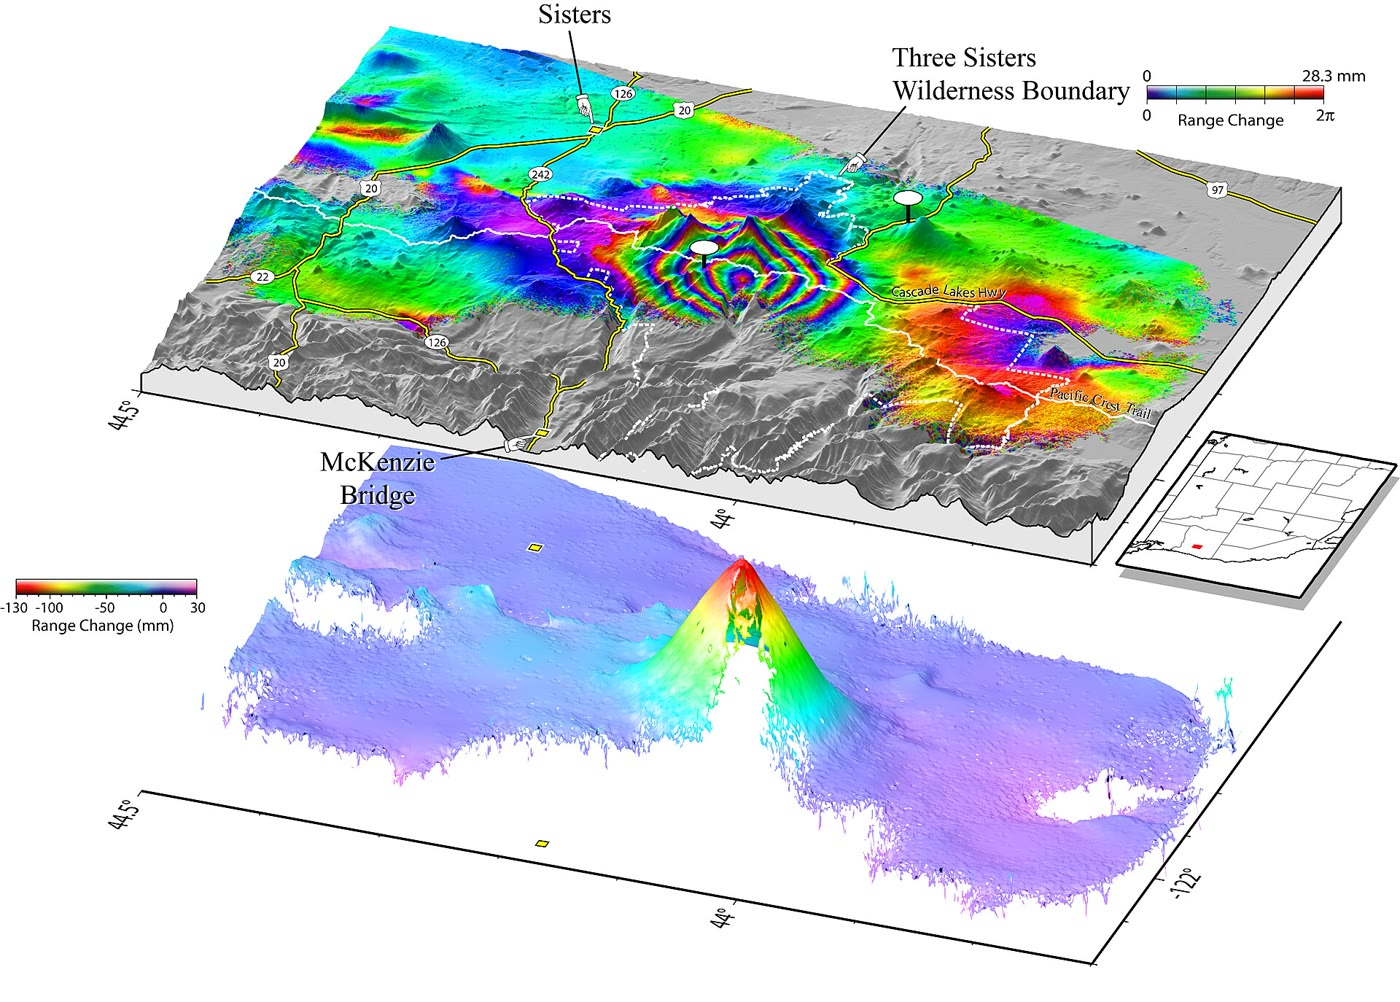
\includegraphics[width=0.86\linewidth]{images/book5/b3-three-sisters-insar.jpg}
\par\smallskip{\small Di atas, \omterm{def:b3:remote-sensing-gis:insar}{interferogram} pusat vulkanik Three Sisters,
Oregon, 1995--2001, ditampilkan di atas relief: setiap siklus warna
adalah \qty{28.3}{mm} perubahan jarak, dan mata banteng berupa cincin di
pusat menandai pengangkatan. Di bawah, data yang sama setelah pembukaan lilitan dan digambar sebagai
relief: jarak memendek hingga \qty{130}{mm} di pusat. U.S.
Geological Survey (Wicks dkk., 2002), domain
publik.}\label{fig:b3:remote-sensing-gis:three-sisters}
\end{omfigure}
% ledger: photo:b3-three-sisters-insar, usgs:insar-fs

\begin{inthelab}[Stasiun darat]
\begin{minipage}[t]{0.55\linewidth}\vspace{0pt}
Satelit pencitra merekam jauh lebih banyak daripada yang dapat dikirimnya saat melintasi
tempat yang dicitranya. Radar satelit Sentinel-1 dapat mencitra
hingga setengah jam setiap orbit dan menyimpan datanya di dalam satelit, hingga
1410 gigabit; ia mengirimkannya ke bawah melalui dua kanal, masing-masing 260 megabit per
detik, sehingga simpanan penuh membutuhkan sekitar 45 menit untuk dikosongkan. Stasiun
darat menerimanya: ketika satelit terbit di atas cakrawala, piringan antena
berputar mengarah kepadanya, mengikutinya melintasi langit, dan melepaskannya ketika ia terbenam,
sementara operator memeriksa bahwa aliran datanya tiba utuh. Data kemudian
dikirim ke pusat pengolahan, tempat gema mentah berubah menjadi citra.
\end{minipage}\hfill
\begin{minipage}[t]{0.42\linewidth}\vspace{0pt}
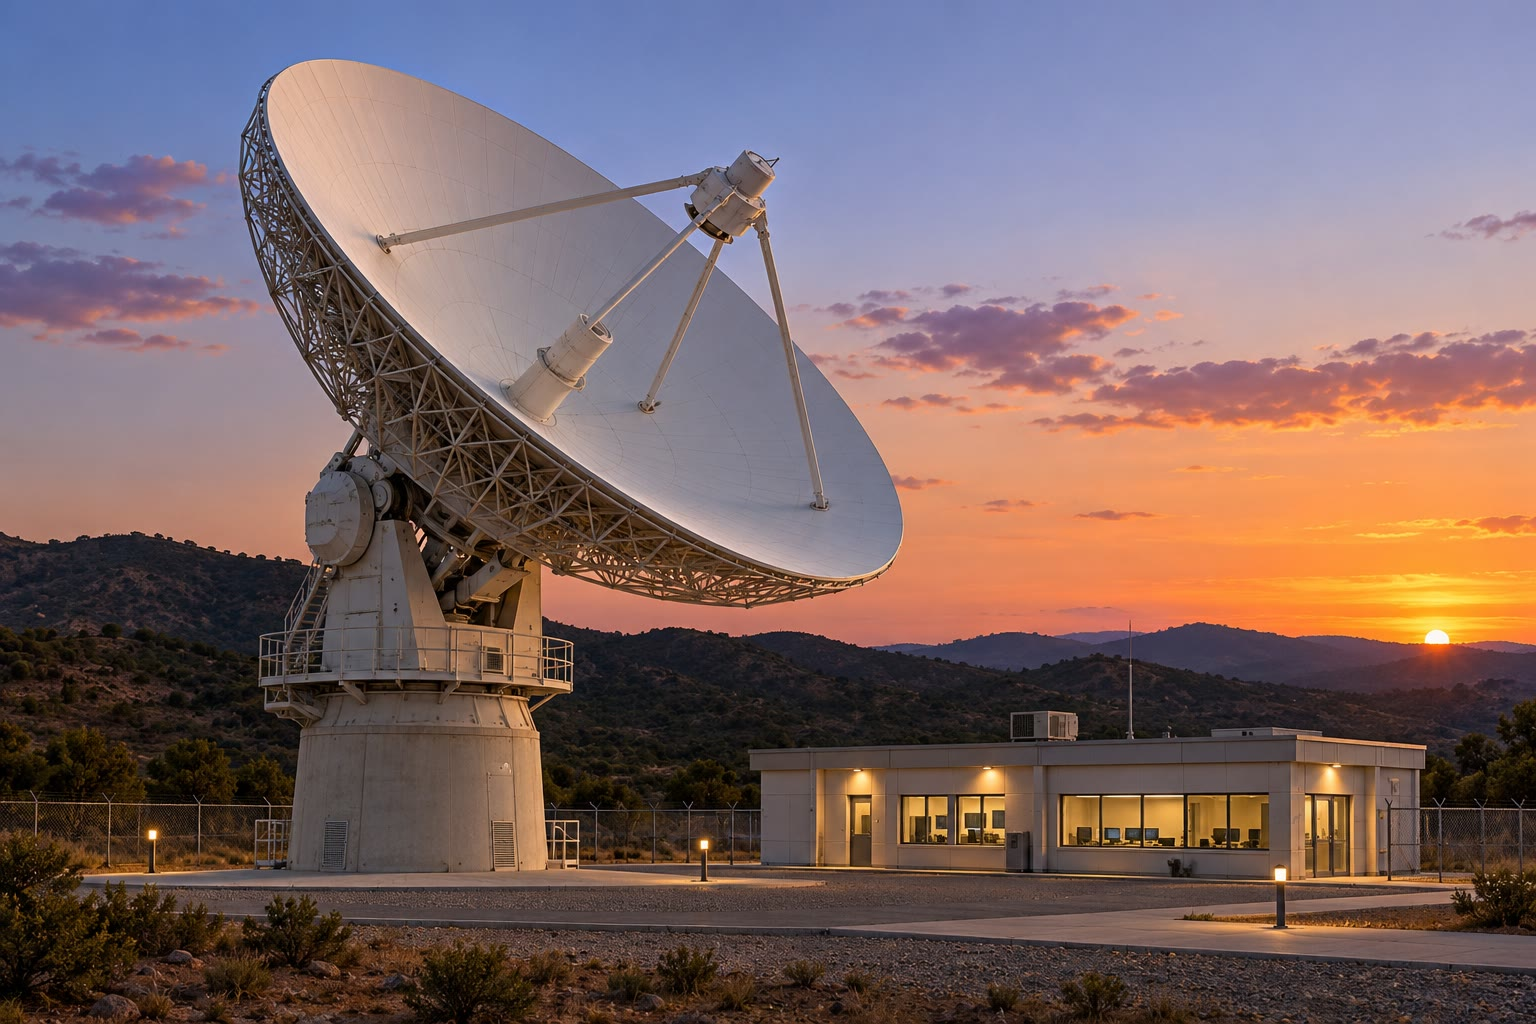
\includegraphics[width=\linewidth]{images/book5/ai/b3-ground-station.jpg}

{\scriptsize Stasiun darat satelit saat senja: piringan pelacak besar dan
gedung operasinya (ilustrasi buatan AI).}
\end{minipage}
\end{inthelab}
% ledger: esa:s1-downlink

\section{Sistem informasi geografis}\label{sec:b3:remote-sensing-gis:gis}

Citra satelit, model elevasi tanah, peta
geologi, sumur, dan jalan adalah lapisan dari satu sistem
informasi geografis, yang menyimpannya dalam satu kerangka koordinat bersama dan
menghitung dengannya.

\begin{definition}[Data raster dan vektor]\label{def:b3:remote-sensing-gis:data-models}
\emph{Data raster}\index{data raster} merepresentasikan suatu lapisan dengan kisi dari
sel, masing-masing menyimpan satu nilai: reflektansi, elevasi, atau kelas.
\emph{Data vektor}\index{data vektor (SIG)} merepresentasikannya dengan titik, garis
dan poligon yang diberikan oleh koordinat titik sudutnya, masing-masing membawa
baris atribut dalam sebuah tabel.
\end{definition}

\begin{omfigure}
\centering
\begin{tikzpicture}[x=0.5cm, y=0.5cm, font=\scriptsize]
\begin{scope}
\draw[black!40] (0,0) rectangle (10,7);
\fill[omSea!50, draw=omDef, thick] (3,4.5) ellipse (1.8 and 1.2);
\draw[omDef, very thick] (4.8,4.5) -- (7,3.5) -- (10,2);
\fill[red!70!black] (7,5.5) circle (0.14); \fill[red!70!black] (2,1.5) circle (0.14);
\node[anchor=south] at (5,7.1) {vektor};
\node at (3,4.5) {danau};
\node[anchor=south west] at (7.1,5.6) {sumur 1};
\node[anchor=south west] at (2.1,1.6) {sumur 2};
\node[anchor=north east] at (9.9,2.2) {sungai};
\end{scope}
\begin{scope}[xshift=6.5cm]
\foreach \i/\j in {1/4,2/4,3/4,4/4,2/3,3/3,2/5,3/5} {\fill[omSea!50] (\i,\j) rectangle ++(1,1);}
\foreach \i/\j in {5/4,6/3,7/3,8/2,9/2} {\fill[omDef!70] (\i,\j) rectangle ++(1,1);}
\foreach \i/\j in {7/5,2/1} {\fill[red!70!black] (\i,\j) rectangle ++(1,1);}
\draw[black!30, step=1] (0,0) grid (10,7);
\draw[black!40] (0,0) rectangle (10,7);
\node[anchor=south] at (5,7.1) {raster};
\end{scope}
\end{tikzpicture}
\par\smallskip{\small Peta yang sama sebagai data vektor (kiri: sebuah poligon, sebuah garis
dan dua titik, tepat posisinya, masing-masing dengan atributnya) dan sebagai
\omterm{def:b3:remote-sensing-gis:data-models}{data raster} (kanan: satu nilai per sel, danau oleh sel yang titik pusatnya berada
di dalamnya, sungai dan sumur oleh sel yang dilintasinya). Raster mudah dihitung
sel demi sel; lapisan vektor mempertahankan bentuk dan topologi pada
skala apa pun.}\label{fig:b3:remote-sensing-gis:raster-vector}
\end{omfigure}

\begin{definition}[Georeferensi]\label{def:b3:remote-sensing-gis:georef}
Yang disebut \emph{georeferensi}\index{georeferensi} adalah pemberian koordinat peta
dalam proyeksi yang dinyatakan ke setiap piksel citra atau setiap
titik sudut gambar, biasanya dengan mencocokkan transformasi pada titik kontrol
tanah yang posisinya diketahui di kedua sistem.
\end{definition}

Untuk raster berorientasi utara dalam kerangka terproyeksi, transformasinya affin:
sel pada kolom $i$ dan baris $j$ memiliki sudutnya di $E = E_0 + i\,\Delta$,
$N = N_0 - j\,\Delta$, dengan $\Delta$ ukuran sel. Citra satelit mula-mula
diresampel ke kisi seperti itu; lapisan dalam proyeksi berbeda
diproyeksikan ke satu proyeksi sebelum digabungkan.

\begin{method}[Lereng, aspek, dan bayangan bukit dari model elevasi digital]\label{met:b3:remote-sensing-gis:slope}
Pada kisi elevasi $z_{i,j}$ dengan jarak $\Delta$ ($i$ ke timur, $j$
ke utara), hitung taksiran gradien dengan selisih pusat,
\[
\frac{\partial z}{\partial x} \approx \frac{z_{i+1,j} - z_{i-1,j}}{2\Delta} ,
\qquad
\frac{\partial z}{\partial y} \approx \frac{z_{i,j+1} - z_{i,j-1}}{2\Delta} .
\]
Yang disebut \emph{lereng} adalah $S = \arctan|\nabla z|$; \emph{aspek} adalah
azimut turun paling curam, yakni arah $-\nabla z$, $A =
\operatorname{atan2}(-\partial z/\partial x, -\partial z/\partial y)$
diukur searah jarum jam dari utara. \emph{Bayangan bukit} untuk cahaya dari
azimut $A_0$ pada sudut zenit $Z$ adalah $\cos Z\cos S + \sin Z\sin S
\cos(A_0 - A)$, yaitu kosinus sudut antara cahaya dan normal
terhadap tanah, diatur nol bila bernilai negatif.
\end{method}

Selisih pusat tepat untuk bidang datar dan keliru sebesar
$\Delta^2 z'''/6$ selain itu; relief teduh Varden Hills dalam
volume Tahun~1 dihitung dengan cara ini, disinari dari barat laut.
Turunan memperbesar galat kisi: model dengan lompatan antarbaris tampak
sebagai garis-garis pada peta lerengnya.

\begin{definition}[Aljabar peta]\label{def:b3:remote-sensing-gis:map-algebra}
Yang disebut \emph{aljabar peta}\index{aljabar peta} adalah perhitungan lapisan raster baru
sel demi sel dari satu atau lebih lapisan pada kisi yang sama: secara aritmetika
(NDVI dari dua pita), secara perbandingan (sel yang lebih curam daripada
\ang{15}), secara logika (dan, atau, tidak), atau dari lingkungan
sel (lereng).
\end{definition}

\begin{definition}[Zona penyangga; tumpang susun]\label{def:b3:remote-sensing-gis:operations}
Yang disebut \emph{zona penyangga}\index{zona penyangga (SIG)} suatu objek pada jarak $d$ adalah
daerah pada peta dalam jarak $d$ darinya. Sebuah
\emph{tumpang susun}\index{tumpang susun (SIG)} menggabungkan dua lapisan atau lebih dari
wilayah yang sama menjadi satu, setiap tempat pada hasil membawa atribut dari
semuanya; pemilihan tempat yang memenuhi beberapa syarat sekaligus
adalah pemakaian yang paling lazim.
\end{definition}

\begin{omfigure}
\centering
\begin{tikzpicture}
\begin{groupplot}[group style={group size=2 by 2, horizontal sep=2.0cm, vertical sep=1.5cm},
  width=0.43\linewidth, axis equal image, enlargelimits=false,
  xmin=0, xmax=10, ymin=0, ymax=8,
  tick label style={font=\scriptsize}, label style={font=\small}, title style={font=\small}]
\nextgroupplot[title={(a) lereng (derajat)}, ylabel={utara (km)}, colormap/viridis,
  point meta min=0, point meta max=24, colorbar right,
  colorbar style={width=0.18cm, ytick={0,5,10,15,20}, tick label style={font=\tiny}, axis equal=false}]
\addplot[matrix plot*, mesh/cols=101, point meta=explicit] table[x=x, y=y, meta=slope] {figdata/out/bachelor-3-varden_gis-grid.dat};
\addplot[white, thick] table {figdata/out/shared-region-river.dat};
\nextgroupplot[title={(b) aspek},
  colormap={aspect}{rgb255=(220,20,30) rgb255=(240,200,0) rgb255=(30,170,60) rgb255=(30,90,220) rgb255=(220,20,30)},
  point meta min=0, point meta max=360, colorbar right,
  colorbar style={width=0.18cm, ytick={0,90,180,270,360}, yticklabels={U,T,S,B,U}, tick label style={font=\tiny}, axis equal=false}]
\addplot[matrix plot*, mesh/cols=101, point meta=explicit] table[x=x, y=y, meta=aspect] {figdata/out/bachelor-3-varden_gis-grid.dat};
\addplot[black, thick] table {figdata/out/shared-region-river.dat};
\nextgroupplot[title={(c) dua lapisan}, xlabel={timur (km)}, ylabel={utara (km)},
  colormap={lay}{rgb255=(245,245,245) rgb255=(150,150,150) rgb255=(225,195,140) rgb255=(120,70,20)},
  colormap access=piecewise constant, point meta min=-0.5, point meta max=3.5,
  legend columns=2, legend style={font=\tiny, at={(0.5,-0.3)}, anchor=north, /tikz/every even column/.append style={column sep=4pt}}]
\addplot[matrix plot*, mesh/cols=101, point meta=explicit, forget plot] table[x=x, y=y, meta=layers] {figdata/out/bachelor-3-varden_gis-grid.dat};
\addplot[omDef, thick, forget plot] table {figdata/out/shared-region-river.dat};
\addlegendimage{area legend, fill={rgb,255:red,150;green,150;blue,150}, draw=black!40}
\addlegendentry{lebih curam daripada \ang{15}}
\addlegendimage{area legend, fill={rgb,255:red,225;green,195;blue,140}, draw=black!40}
\addlegendentry{serpih}
\addlegendimage{area legend, fill={rgb,255:red,120;green,70;blue,20}, draw=black!40}
\addlegendentry{keduanya}
\nextgroupplot[title={(d) tumpang susun}, xlabel={timur (km)},
  colormap={cls}{rgb255=(245,245,245) rgb255=(225,195,140) rgb255=(190,150,90) rgb255=(200,20,30)},
  colormap access=piecewise constant, point meta min=-0.5, point meta max=3.5,
  legend columns=2, legend style={font=\tiny, at={(0.5,-0.3)}, anchor=north, /tikz/every even column/.append style={column sep=4pt}}]
\addplot[matrix plot*, mesh/cols=101, point meta=explicit, forget plot] table[x=x, y=y, meta=class] {figdata/out/bachelor-3-varden_gis-grid.dat};
\addplot[omDef, thick, forget plot] table {figdata/out/shared-region-river.dat};
\addplot[black, thin, dashed, unbounded coords=jump] table[x=x, y=y] {figdata/out/bachelor-3-varden_gis-buffer.dat};
\addlegendentry{zona penyangga \qty{1}{km}}
\addlegendimage{area legend, fill={rgb,255:red,225;green,195;blue,140}, draw=black!40}
\addlegendentry{serpih}
\addlegendimage{area legend, fill={rgb,255:red,190;green,150;blue,90}, draw=black!40}
\addlegendentry{serpih dalam zona penyangga}
\addlegendimage{area legend, fill={rgb,255:red,200;green,20;blue,30}, draw=black!40}
\addlegendentry{terpilih}
\end{groupplot}
\end{tikzpicture}
\par\smallskip{\small Sesi SIG di Varden Hills, dari model elevasinya
pada kisi \qty{100}{m}. (a)~Lereng, hingga \ang{23} di sisi
lembah; (b)~aspek, arah yang dihadap tanah, kedua sisi sungai yang
saling berhadapan; (c)~dua lapisan, sel yang lebih curam daripada \ang{15}
dan singkapan serpih Jurassik; (d)~\omterm{def:b3:remote-sensing-gis:operations}{tumpang susunnya} dengan
\omterm{def:b3:remote-sensing-gis:operations}{zona penyangga} \qty{1}{km} sungai (putus-putus): \qty{0.32}{km^2} serpih curam
di atas sungai, saringan awal untuk tanah yang mungkin
longsor.}\label{fig:b3:remote-sensing-gis:varden}
\end{omfigure}

Gambar di atas menjalankan seluruh rantai: \omterm{def:b3:remote-sensing-gis:map-algebra}{aljabar peta} pada kisi elevasi
menghasilkan lereng dan aspek; perbandingan mengubah lereng menjadi lapisan
sel-sel curam; peta geologi memberikan serpih; \omterm{def:b3:remote-sensing-gis:operations}{zona penyangga} sungai
memberikan lapisan ketiga; irisannya, \omterm{def:b3:remote-sensing-gis:operations}{tumpang susun} dengan operator logika \emph{dan},
menyisakan 32 sel dari 8181. Jawaban hanya sebaik lapisannya: pada kisi
yang lebih kasar, lereng tampak lebih landai dan lebih sedikit sel yang lolos.

\begin{definition}[Klasifikasi terbimbing; matriks konfusi]\label{def:b3:remote-sensing-gis:classification}
Yang disebut \emph{klasifikasi terbimbing}\index{klasifikasi terbimbing} menetapkan setiap piksel citra
ke salah satu dari sekumpulan kelas, berdasarkan aturan atau statistik
yang dipelajari dari piksel latih yang kelasnya diketahui di lapangan.
Hasilnya berupa \emph{matriks konfusi}\index{matriks konfusi} yang menghitung, untuk
sekumpulan piksel acuan yang terpisah, berapa banyak piksel tiap kelas sebenarnya yang ditetapkan ke tiap kelas:
$n_{ij}$ piksel yang diklasifikasikan sebagai $i$ sebenarnya termasuk $j$.
\end{definition}

Diagonal memuat piksel yang diklasifikasikan dengan benar. Dengan $N$ piksel acuan,
\emph{akurasi keseluruhan} adalah $\sum_i n_{ii}/N$. \emph{Akurasi
pengguna} suatu kelas, yaitu $n_{ii}$ dibagi jumlah barisnya, adalah peluang bahwa
piksel yang dipetakan sebagai $i$ memang $i$; \emph{akurasi produsen}, $n_{ii}$ dibagi
jumlah kolomnya, adalah peluang bahwa $i$ sebenarnya dipetakan sebagai $i$. Koefisien
\emph{kappa} membandingkan akurasi keseluruhan $p_o$ dengan
akurasi $p_e = \sum_i (\text{baris}_i)(\text{kolom}_i)/N^2$ yang akan dicapai
penetapan acak dengan total yang sama: $\kappa = (p_o - p_e)/(1 -
p_e)$.

\begin{center}
\small
\begin{tabular}{l|ccc|c}
\hline
diklasifikasikan \textbackslash{} acuan & air & hutan & batuan terbuka & jumlah \\
\hline
air & 45 & 2 & 0 & 47 \\
hutan & 3 & 38 & 7 & 48 \\
batuan terbuka & 0 & 5 & 30 & 35 \\
\hline
jumlah & 48 & 45 & 37 & 130 \\
\hline
\end{tabular}
\end{center}

Dalam contoh rekaan ini, 113 dari 130 piksel benar, akurasi keseluruhan
sebesar \qty{86.9}{\percent}. Hutan memiliki akurasi pengguna sebesar
$38/48 = \qty{79}{\percent}$, tetapi akurasi produsen $38/45 =
\qty{84}{\percent}$: tujuh piksel batuan terbuka, mungkin dalam bayangan, dipetakan sebagai hutan.
Penetapan acak akan mencapai $p_e = 0.338$, dan $\kappa =
0.80$.

\section{Latihan}

\begin{exercise}[$\star$]\label{exo:b3:remote-sensing-gis:1}
Sebuah lahan memiliki reflektansi 0.06 pada pita merah dan 0.42 pada
pita inframerah dekat milik sebuah pencitra; lahan yang dibajak di sebelahnya 0.21 dan
0.28. Hitung NDVI keduanya, lalu jelaskan apa yang disiratkan tiap nilai.
\end{exercise}

\begin{exercise}[$\star$]\label{exo:b3:remote-sensing-gis:2}
Pencitra Landsat~8 meliputi jalur selebar \qty{185}{km} dengan piksel \qty{30}{m},
dan pita pankromatiknya dengan piksel \qty{15}{m}. (a)~Berapa banyak
piksel yang dimuat sebaris melintasi jalur di tiap kasus? (b)~Berapa tingkat
yang dihasilkan 12 bit dan 8 bit? (c)~Berapa \omterm{def:b3:remote-sensing-gis:resolutions}{waktu kunjungan ulang} Landsat~8
sendiri, dan Landsat 8 dan 9 bersama-sama?
\end{exercise}

\begin{exercise}[$\star$]\label{exo:b3:remote-sensing-gis:3}
(a)~Pada \omterm{def:b3:remote-sensing-gis:insar}{interferogram} Sentinel-1 ($\lambda = \qty{5.55}{cm}$) suatu
cekungan yang mengalami penurunan, enam jalur interferensi memisahkan tepi stabil dari pusatnya.
Berapa perubahan garis pandang di pusat? (b)~Berapa nilai satu
jalur itu untuk satelit yang lebih tua dengan panjang gelombang \qty{5.66}{cm}?
\end{exercise}

\begin{exercise}[$\star$]\label{exo:b3:remote-sensing-gis:4}
Sebuah altimeter laser berada \qty{500}{km} di atas tanah. (a)~Berapa lama sebuah pulsa
perlu untuk kembali? (b)~Jika waktu tiap foton dicatat hingga \qty{800}{ps}, seberapa
teliti satu pengukuran jarak?
\end{exercise}

\begin{exercise}[$\star\star$]\label{exo:b3:remote-sensing-gis:5}
Sebuah piksel pita~10 Landsat~8 (ambil $\lambda = \qty{10.9}{\micro\metre}$)
setelah \omterm{def:b3:remote-sensing-gis:atm-correction}{koreksi atmosfer}, memiliki radiansi spektral sebesar
\qty{9.0}{W.m^{-2}.sr^{-1}.\micro\metre^{-1}}. (a)~Hitung \omterm{def:b3:remote-sensing-gis:brightness}{suhu kecerahannya}.
(b)~Permukaannya berupa padang rumput dengan emisivitas 0.98: berapa
suhu kinetiknya?
\end{exercise}

\begin{exercise}[$\star\star$]\label{exo:b3:remote-sensing-gis:6}
Radar Sentinel-1 terbang \qty{693}{km} di atas dengan antena sepanjang \qty{12.3}{m}
pada $\lambda = \qty{5.55}{cm}$. (a)~Dengan mengabaikan kelengkungan Bumi, hitung
jangkauan miring ke titik yang terlihat pada sudut datang
\ang{35}. (b)~Berapa resolusi azimut yang diberikan antena nyata sepanjang itu
di sana, dan berapa yang diberikan apertur sintetik? (c)~Berapa panjang
apertur sintetik?
\end{exercise}

\begin{exercise}[$\star\star$]\label{exo:b3:remote-sensing-gis:7}
Sebuah jendela $3\times3$ dari model elevasi digital dengan sel \qty{30}{m}
terbaca dengan utara di atas,
\[
\begin{matrix} 412 & 418 & 425 \\ 405 & 410 & 418 \\ 398 & 401 & 409 \end{matrix}
\qquad (\unit{m}).
\]
Dengan selisih terpusat pada sel pusat, hitung lereng, aspek
dan naungan bukit untuk cahaya dari barat laut, \ang{45} di atas
cakrawala.
\end{exercise}

\begin{exercise}[$\star\star$]\label{exo:b3:remote-sensing-gis:8}
Sebuah peta penutup lahan diperiksa terhadap 160 piksel acuan (baris: peta;
kolom: kenyataan; kelas air, hutan, lahan pertanian, kota):
\[
\begin{pmatrix} 48 & 3 & 1 & 0 \\ 4 & 37 & 6 & 1 \\ 2 & 5 & 29 & 2 \\ 0 & 1 & 2 & 19 \end{pmatrix} .
\]
Hitung akurasi keseluruhan, serta akurasi pengguna dan akurasi produsen tiap
kelas, dan kappa. Kelas mana yang paling sering terlewatkan?
\end{exercise}

\begin{exercise}[$\star\star$]\label{exo:b3:remote-sensing-gis:9}
Sebuah piksel termal \qty{100}{m} memuat aliran lava segar pada \qty{1443}{K}
menutupi \qty{4}{\percent} darinya; sisanya berupa tanah pada \qty{290}{K}; anggap
keduanya sebagai benda hitam. (a)~Hitung temperatur kecerahan piksel pada
\qty{10.9}{\micro\metre} dan bandingkan dengan temperatur rata-rata.
(b)~Hitung rasio radiansi benda hitam dari lava dan
tanah pada \qty{2.2}{\micro\metre}, serta temperatur kecerahan piksel
di sana. Pita mana yang lebih baik mendeteksi lava?
\end{exercise}

\begin{exercise}[$\star\star\star$]\label{exo:b3:remote-sensing-gis:10}
Dua \omterm{def:b3:remote-sensing-gis:insar}{interferogram} dari deformasi yang sama dibuat dari dua lintasan, satu
dengan satelit di timur tanah dan satu lagi dengan satelit di barat,
keduanya pada sudut datang \ang{35}. Di satu titik, garis
pandang memendek sebesar \qty{64}{mm} pada yang pertama dan \qty{38}{mm} pada
yang kedua. Dengan asumsi tidak ada gerak utara--selatan, hitung perpindahan vertikal dan
perpindahan ke timur. Mengapa satu lintasan tidak cukup?
\end{exercise}

\begin{exercise}[$\star\star\star$]\label{exo:b3:remote-sensing-gis:11}
\omterm{def:b3:remote-sensing-gis:insar}{Pembukaan lilitan fase} gagal di tempat fase melompat lebih dari $\pi$ antara
piksel bertetangga. (a)~Tunjukkan bahwa garis pandang harus berubah kurang dari
$\lambda/4$ dari satu piksel ke piksel berikutnya, \qty{13.9}{mm} untuk
Sentinel-1. (b)~Untuk sumber Mogi pada $z_0 = \qty{4}{km}$ dengan $\Delta V =
\qty{e7}{m^3}$ dan $\nu = 0.25$, dilihat secara vertikal, tunjukkan bahwa
gradien $u_z$ terbesar berada pada $r = z_0/2$ dan hitung nilainya. (c)~Berapa
ukuran piksel terbesar yang masih membuat pinggiran dapat dibedakan?
\end{exercise}

\begin{exercise}[$\star\star\star$]\label{exo:b3:remote-sensing-gis:12}
(a)~Tunjukkan bahwa NDVI berada di antara $-1$ dan $+1$ untuk
reflektansi nonnegatif, dan bahwa nilainya tetap jika kedua reflektansi
dikalikan faktor yang sama. (b)~Rumput memiliki reflektansi 0.051 (merah)
dan 0.502 (inframerah dekat). Citra yang belum dikoreksi menambahkan radiansi lintasan
setara dengan 0.03 pada merah dan 0.01 pada inframerah dekat. Hitung
NDVI dengan dan tanpa koreksi itu. (c)~Apa implikasinya bagi peta NDVI
yang dibuat dari citra yang belum dikoreksi pada hari berkabut?
\end{exercise}

\section{Soal: Lereng yang menggelembung di Gunung Halvren}

\begin{problem}[{Soal akhir pekan --- vegetasi, panas dan radar
interferogram pada gunung api rekaan}]
\label{pb:b3:remote-sensing-gis:1}
Gunung Halvren, gunung api rekaan, pernah meletus dan membentuk aliran lava pada 1890, 1960
dan 2005 ke lerengnya yang berhutan. Medan fumarol mengepulkan uap di puncaknya.
Data satelit dari tahun terbaru diberikan di bawah.

\medskip\noindent\textbf{Bagian I --- Vegetasi pada aliran lava.} Reflektansi terkoreksi
pada pita merah dan inframerah dekat:
\begin{center}
\small
\begin{tabular}{lcccc}
\hline
permukaan & hutan & aliran 1890 & aliran 1960 & aliran 2005 \\
\hline
merah & 0.04 & 0.07 & 0.11 & 0.12 \\
inframerah dekat & 0.38 & 0.30 & 0.21 & 0.14 \\
\hline
\end{tabular}
\end{center}
\begin{enumerate}
\item Hitung NDVI keempat permukaan.
\item Urutkan aliran berdasarkan pemulihan vegetasinya. Apakah urutan itu
  sama dengan urutan umurnya?
\item Mengapa NDVI aliran 2005 tidak nol, padahal hampir
  tidak ada yang tumbuh di atasnya?
\item Mengapa NDVI lebih andal daripada reflektansi inframerah dekat
  saja pada lereng curam dengan penyinaran tidak merata di gunung api?
\end{enumerate}

\medskip\noindent\textbf{Bagian II --- Medan fumarol.} Pada pita termal
(ambil $\lambda = \qty{10.9}{\micro\metre}$) radiansi terkoreksi dari
sebuah piksel \qty{100}{m} di dataran tinggi puncak yang jauh dari fumarol adalah
\qty{8.40}{W.m^{-2}.sr^{-1}.\micro\metre^{-1}}, dan radiansi piksel di atas
medan fumarol \qty{9.95}{W.m^{-2}.sr^{-1}.\micro\metre^{-1}}.
\begin{enumerate}[resume]
\item Hitung temperatur kecerahan kedua piksel itu.
\item Batuan dataran tinggi memiliki emisivitas 0.97. Berapa
  temperatur kinetiknya?
\item Lubang fumarol dan tanah hangat di sekitarnya berada pada
  \qty{370}{K}. Anggap keduanya dan sisa piksel sebagai benda hitam,
  sisanya pada radiansi dataran tinggi, berapa bagian piksel yang mereka
  tutupi, dan berapa luasnya?
\item Mengapa temperatur rata-rata berbobot luas piksel lebih rendah
  daripada temperatur kecerahannya?
\end{enumerate}

\medskip\noindent\textbf{Bagian III --- Interferogram.} Dua citra Sentinel-1
($\lambda = \qty{5.55}{cm}$, sudut datang \ang{35}, satelit di sebelah
timur) yang diambil dengan selang 48 hari menunjukkan pola sasaran di lereng timur. Dari
area stabil ke pusat pola terhitung lima pinggiran penuh dan
empat persepuluh pinggiran keenam, semuanya dalam arah gerak menuju
satelit.
\begin{enumerate}[resume]
\item Mengapa dua citra harus diambil dari posisi yang hampir sama, dan berapa
  siklus orbit satu satelit yang memisahkan keduanya?
\item Hitung perubahan garis pandang di pusat.
\item Di pusat, tanah bergerak hanya secara vertikal. Hitung pengangkatan
  di sana.
\item Jelaskan mengapa pola itu tidak berbentuk lingkaran, dan di sisi mana,
  timur atau barat, pinggirannya paling rapat.
\item Sepanjang garis utara--selatan melalui pusat, perubahan garis
  pandang turun menjadi setengah nilai pusatnya pada jarak \qty{3.4}{km} dari
  pusat. Mengapa memakai garis itu, dan kedalaman berapa yang diberikannya untuk
  sumber Mogi?
\item Berapa pinggiran yang memisahkan pusat dari titik setengah nilai itu?
\item Uap air di udara dapat menunda gelombang radar secara berbeda pada
  kedua tanggal dan membentuk pinggirannya sendiri. Bagaimana \omterm{def:b3:remote-sensing-gis:insar}{interferogram} kedua,
  dari pasangan tanggal lain, membantu membedakan keduanya?
\end{enumerate}

\medskip\noindent\textbf{Bagian IV --- Volume.} Ambil $\nu = 0.25$.
\begin{enumerate}[resume]
\item Dari $u_z(0) = (1 - \nu)\Delta V/(\pi z_0^2)$, hitung perubahan
  volume sumber itu.
\item Nyatakan sebagai laju rata-rata per hari dan per tahun selama 48 hari.
\item Hitung perpindahan horizontal terbesar dan di mana itu terjadi.
\item Jika reservoar berbentuk bola dengan jari-jari $z_0/3$, berapa besar
  volumenya, dan perubahan itu mewakili berapa bagian darinya?
\item Ukuran berhingga bola dengan jari-jari $z_0/3$ mengubah pengangkatan
  sekitar \qty{3}{\percent}. Apakah itu mengubah jawaban pertanyaan~16
  secara berarti, mengingat ketelitian penghitungan pinggiran?
\item Pengamatan lain apa, dari Bagian I dan II atau dari lapangan,
  akan mendukung interpretasi reservoar yang sedang terisi?
\item Berikan perubahan volume reservoar di bawah Gunung Halvren, dalam
  juta meter kubik, dengan dua angka penting.
\end{enumerate}
\end{problem}
% ledger: nasa:ndvi, esa:s1-sar, esa:s1-orbit, esa:s1-iw, dmodels:mogi, dmodels:mogi-radial, const:h, const:c, const:kB
